\section{Experiments}
\label{sec:experiments}

We evaluate the two operations separately: storing a growing history with updates and revisable identities, and reading only the evidence required by a question.

\subsection{Evaluation setup}
\label{sec:setup}

We use four public benchmarks. The primary MemoryAgentBench (MAB) evaluation uses a paired 767-question sample over 10 task groups and 59 documents, extended on Align+ to 1{,}074 questions over 14 task groups (full set: 3{,}671 questions over 29 task groups); all MAB scores use the official scorer\footnote{The scorer used for these runs is fixed at commit \texttt{455306d}.} with Kimi-K3 as answerer. For LongMemEval, the complete conversation set is written first, and the three answer methods use paired $n{=}25/25/27$ samples. MAB reports percentages (100 all correct, 0 none); AR is \emph{Accurate Retrieval}, TTL \emph{Test-Time Learning}, LRU \emph{Long-Range Understanding}, SF \emph{Selective Forgetting}; MCC is \emph{Multi-Class Classification}, Recom is movie recommendation scored by Recall@5, and FC-SH/FC-MH are single-hop and multi-hop FactConsolidation; Recall, $J$, exact-match, and Overall are higher-is-better, while calls, tokens, and bytes are costs. Sampling and judging details are in Appendix~\ref{app:sampling}, and Appendix Table~\ref{tab:experiment-map} maps each benchmark to the storage or reading question.

\begin{figure*}[t]
  \centering
  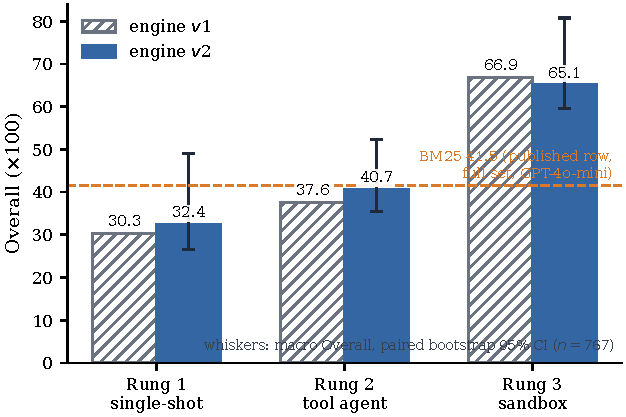
\includegraphics[width=\textwidth]{figures/fig2_ladder.pdf}
  \caption{MemoryAgentBench results by method and task (official scorer, Kimi-K3 answerer). (a) Overall scores: Base on the frozen paired sample ($n{=}767$), Align+ on the extended sample ($n{=}1074$), with marginal 95\% bootstrap intervals; (b) Align+ domain scores at the extended sample; (c) selected task scores; (d) all 209 residual zero-score items of the extended sample. The two sample definitions are labeled separately.}
  \label{fig:ladder}
\end{figure*}

\subsection{How to store: updates and entity alignment}
\label{sec:temporal-benchmark}
\label{sec:engine-versions}
\label{sec:engine-paired}
\label{sec:deletion-boundary}

LongMemEval asks whether an earlier statement and a later correction can both be found after the complete conversation history has been written. In paired runs, direct retrieval changes from 0.68 to 0.72, memory-tool reading changes from 0.68 to 0.72, and source-grounded reading changes from 0.889 to 0.926 ($n{=}25/25/27$; these tracks are small and directional). Together, these paired runs indicate that old and new observations remain jointly accessible to the read path. The separate 500-question LongMemEval-S run reaches 84.60\% with Qwen3.7-plus as both answerer and judge; this protocol differs from the other answerer/judge pairings in the table.

The alignment comparison tests when identity is finalized. Immediate alignment decides window by window; delayed alignment waits for the surrounding evidence. In the paired ingest records, calls fall from 609 to 329 per MAB document and from 63.8 to 22.0 per LongMemEval document. Same-name duplicate families fall from 340 to 124 on MAB and from 482 to 99 on LongMemEval. MCC and FC-MH each increase by 3 points in the paired sample (95\% interval $-7$ to $+13$, including zero). These measurements cover the revised write path, which combines delayed alignment with batched or concurrent processing; its practical effect is lower construction cost with more opportunity to revise identity links. The three-arm breakdown is reported in Appendix Table~\ref{tab:alignment-ab}, and Appendix Figure~\ref{fig:alignment-outcomes} separates its cost, duplicate-family, and quality changes.

MEME separates historical retention from deletion: on 100 episodes (694 after-task checks), deletion accuracy is 0\%, cascade 46.34\%, and absence 59.23\%. The zero is a property of the evaluated write/read path: a MEME deletion event asks the system to stop returning one earlier fact while keeping the surrounding history, and the tested path records that statement as another observation, with no tombstone or query-time suppression rule that propagates from an entity or relation to the affected spans---the evidence is preserved but still retrieved. Supporting deletion requires recording the deletion target, propagating it to derived pointers, and distinguishing current from historical queries. The result locates the missing operation precisely; it is not evidence that source preservation alone implements forgetting. Appendix Figure~\ref{fig:diagnostics} gives the corresponding update, neighbor-hop, and deletion breakdown.

\subsection{How to read: progressive evidence retrieval}
\label{sec:ladder}
\label{sec:relational-benchmark}

Figure~\ref{fig:ladder} gives the panel-level result. Panel (a) rises from about 33 to 40 and then to 71 on Align+; panel (b) shows the source path reaching 88.8 AR, 52.9 TTL, 62.3 LRU, and 80.0 SF while the other paths remain at 2.6 TTL. Panel (c) shows the same advantage on MCC (46.0) and FC-MH (70.0), while panel (d) locates 122 of 209 zero-score questions in TTL. The pattern is consistent with source access and continued evidence gathering for updates and fact consolidation.

The three paths (\cref{sec:answer-paths}) differ in what reaches the answerer and who may request more. \textbf{Fixed retrieval} materializes one ranked list of memory records and chunks that cannot be changed, reopened, or checked. \textbf{Memory-tool reading} may issue several read-only calls, so the second call can use an entity or relation returned by the first, but its context is bounded to returned records with no source-file gate. \textbf{Source-grounded reading} selects document groups with the same index, then opens the original files and sends only gate-accepted spans to the answerer. Thus the second path is adaptive navigation over stored records, while the third is adaptive navigation followed by a source-text read.

The table gives the same pattern row by row: source reading is strongest on MCC, FC-MH, MH-QA, and LongMemEval-S, while tool reading mainly helps tasks such as DetectiveQA. These are the cases in which a relevant-looking first chunk is insufficient: the agent must combine mentions, follow an update, or verify an exact qualifier. The fixed path cannot request the missing mention; the tool path can request another bounded record; source reading can inspect the selected file and verify the wording. Appendix Figure~\ref{fig:alignment} and Appendix Table~\ref{tab:answer-path-differences} provide the 614-question heatmap and the path-level protocol comparison.

The full-context reference reaches 78.7 on 614 questions whose document groups fit its budget. Source-grounded reading reaches 70.8 on those same questions and 71.0 on the expanded 1,074-question sample; it also remains applicable to the 460 questions that exceed the budget. Full context is strong when it fits, whereas addressed reading continues after the corpus outgrows one window.

LoCoMo tests cross-Episode evidence under the Mem0-compatible binary $J$ (the percentage of answers an LLM judge marks correct). Deep-Dream reaches 95.19\% overall (97.38 single-hop, 93.62 multi-hop, 80.21 open-domain, 95.33 temporal), and an independent Qwen3.7-plus cross-judge gives 94.22\% on the same answers. We report this as a single-run diagnostic because 1,529 of 1,540 rows predate runtime-code fingerprinting; the published Mem0 and Zep rows retain their own answerers, judges, and test procedures. The multi-hop and temporal results fit the design: relation paths connect Episodes while source observations retain the supporting statements.

\begin{table*}[t]
\centering
\footnotesize
\setlength{\tabcolsep}{4.5pt}
\renewcommand{\arraystretch}{1.12}
\begin{tabular*}{\textwidth}{@{\extracolsep{\fill}}lrrrrrrr@{}}
\toprule
 & \multicolumn{2}{c}{Direct retrieval}
 & \multicolumn{2}{c}{Tool-assisted reading}
 & \multicolumn{2}{c}{Source reading}
 & \multicolumn{1}{c}{\shortstack{Source$-$Direct\\(Align+)}} \\
\cmidrule(lr){2-3}\cmidrule(lr){4-5}\cmidrule(lr){6-7}\cmidrule(lr){8-8}
Task / domain
 & Base & Align+ & Base & Align+ & Base & Align+
 & \shortstack{Source$-$Direct\\(Align+)} \\
\midrule
\rowcolor{blue!10}
\multicolumn{8}{@{}l}{\textbf{AR: Accurate Retrieval}} \\
SH-QA
 & 54.0 & 48.0 & 84.0 & 72.0 & \textbf{94.0} & \underline{92.0} & 44.0 \\
MH-QA$^{\ddagger}$
 & -- & 22.0 & -- & \underline{42.0} & -- & \textbf{77.0} & 55.0 \\
LongMemEval-S$^{*}$
 & 26.7 & 41.7 & 43.3 & 51.7 & \textbf{90.0} & \underline{88.3} & 46.6 \\
EventQA
 & \underline{90.3} & 89.7 & \underline{90.7} & 88.3 & \textbf{98.0} & \textbf{98.0} & 8.3 \\
\midrule
\rowcolor{green!10}
\multicolumn{8}{@{}l}{\textbf{TTL: Temporal and Test-time Learning}} \\
MCC, icl\_clinic150
 & 4.0 & 2.0 & 3.0 & 2.0 & \underline{43.0} & \textbf{46.0} & 44.0 \\
Recom$^{\ddagger}$
 & -- & \underline{3.2} & -- & \underline{3.2} & -- & \textbf{59.8} & 56.6 \\
\midrule
\rowcolor{orange!12}
\multicolumn{8}{@{}l}{\textbf{LRU: Long-range Understanding}} \\
$\infty$Bench-Sum$^{\dagger}$
 & 0.0 & 0.0 & \underline{28.4} & \textbf{29.8} & 21.2 & 0.0 & 0.0 \\
DetectiveQA
 & 50.0 & \underline{66.7} & 50.0 & \textbf{83.3} & \textbf{83.3} & \textbf{83.3} & 16.6 \\
\midrule
\rowcolor{purple!10}
\multicolumn{8}{@{}l}{\textbf{SF: Selective Forgetting}} \\
FC-SH
 & \underline{68.0} & 66.0 & 67.0 & 63.0 & \textbf{90.0} & \textbf{90.0} & 24.0 \\
FC-MH
 & 2.0 & 3.0 & 4.0 & 4.0 & \underline{67.0} & \textbf{70.0} & 67.0 \\
\midrule
\rowcolor{gray!12}
\textbf{Overall ($n=767$)}
 & 30.2 & 32.4 & 37.6 & 40.7 & \textbf{66.9} & \underline{65.1} & 32.7 \\
Overall ($n{=}1074$, extended)
 & -- & 33.3 & -- & 40.0 & -- & \textbf{71.0} & 37.7 \\
\bottomrule
\end{tabular*}
\caption{MemoryAgentBench scores (percent). The last column is Source$-$Direct within Align+; it is reported when both Align+ paths are available. Bold and underlining mark the best and second-best entry within each row.}
\label{tab:main-results}
\end{table*}



\begin{figure*}[t]
  \centering
  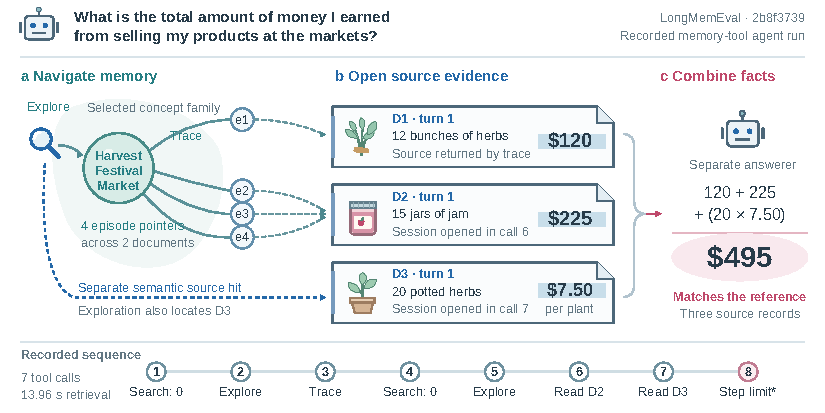
\includegraphics[width=0.88\textwidth]{figures/fig4_agent_trace.pdf}
  \caption{Recorded LongMemEval trace (question \texttt{2b8f3739}): concept tracing exposes four episode pointers across two documents, and semantic retrieval locates the third sales record. Seven successful calls read $120$, $225$, and $7.50$; a malformed eighth response reaches the step limit, after which a separate answerer computes $495$. The trace shows graph navigation locating candidates and source spans supplying the arithmetic.}
  \label{fig:agent-trace}
\end{figure*}


A single recorded trace makes the storage--reading boundary observable. The agent first follows concept and relation pointers across two documents, then opens source spans containing \$120, \$225, the quantity 20, and the \$7.50 unit price and computes $120+225+(20\times7.50)=495$. The seven successful calls show how the graph locates candidates while source spans supply the arithmetic; the malformed eighth response is retained as an audit detail. This case study illustrates the control flow and does not replace aggregate benchmark results.

\subsection{Comparison with existing memory systems}
\label{sec:cross-system}

Table~\ref{tab:main-cross-system} places Deep-Dream beside published results for MAB, LoCoMo, and LongMemEval-S; the model columns make each pairing explicit. In the MAB rows, Kimi-K3 is held fixed: 33.3 with one fixed retrieval result, 40.0 with iterative memory-tool reading, 71.0 with source reading, and the 78.7 full-context row is the same-model upper reference on the 614 questions whose documents fit the window. The published rows retain their reported answerers and judges, so only the same-model MAB pair is a controlled comparison. Category-level reproductions are in Appendix Tables~\ref{tab:mem0-baselines}--\ref{tab:zep-longmemeval} and~\ref{tab:mem0-f1-bleu}. Green rows mark recent strong-model reports: $\dagger$ uses GPT-5-mini/GPT-5, $\ddagger$ uses GPT-4.1-mini or GPT-5-mini with GPT-4o-mini judging, and $\ast$ uses Gemini-3 Pro with GPT-OSS-120B memory and judging \citep{ji2026infini,wang2026memmachine,latimer2025hindsight}. On LongMemEval-S, Deep-Dream's 84.6 (Qwen3.7-plus answerer and judge) is below MemMachine (93.0), Hindsight (91.4), and Supermemory (85.2): the gaps concentrate in session preference, temporal reasoning, and multi-session questions, while Deep-Dream is strong on assistant facts, user facts, and knowledge updates---the next reading and update targets, with the source-reading strength on MAB and the multi-hop and temporal strength on LoCoMo preserved.

For Infini Memory-A, the MAB row uses the four category averages reported in its paper: 81.2 for AR, 51.0 for TTL, 68.6 for LRU, and 58.0 for SF, with 64.7 overall; its finer subtask scores are not substituted for the category values.

\begin{table*}[t]
\centering
\scriptsize
\setlength{\tabcolsep}{2.4pt}
\renewcommand{\arraystretch}{0.82}
{\footnotesize\textbf{(a) MemoryAgentBench (official scorer)}}\\[1.5pt]
\begin{tabular*}{\textwidth}{@{\extracolsep{\fill}}>{\raggedright\arraybackslash}p{0.25\textwidth}>{\raggedright\arraybackslash}p{0.15\textwidth}rrrrr@{}}
\toprule
Memory system & Answerer & AR & TTL & LRU & SF & Overall \\
\midrule
Full context & GPT-4o & 58.1 & 50.0 & 54.9 & 32.5 & 48.8 \\
Full context & GPT-4o-mini & 49.2 & 48.6 & 46.2 & 25.0 & 42.2 \\
Full context & GPT-4.1-mini & 71.8 & 46.2 & 49.1 & 20.5 & 46.9 \\
Full context & Gemini-2.0-Flash & 65.1 & 46.4 & 41.6 & 16.5 & 42.4 \\
Full context & Claude-3.7-Sonnet & 59.7 & 53.9 & 62.2 & 22.5 & 49.6 \\
\rowcolor{blue!9}
Full context ($n{=}614$) & Kimi-K3 & \textbf{96.8} & \textbf{75.0} & 65.2 & 78.0 & \textbf{78.7} \\
\midrule
BM25 RAG & GPT-4o-mini & 60.5 & 44.5 & 35.6 & 25.5 & 41.5 \\
HippoRAG-2 & GPT-4o-mini & 65.1 & 35.8 & 36.2 & 29.5 & 41.6 \\
MIRIX & GPT-4.1-mini & 63.0 & 35.7 & 40.5 & 11.5 & 37.7 \\
MemGPT & GPT-4o-mini & 34.3 & 40.8 & 22.4 & 15.5 & 28.3 \\
Zep & GPT-4o-mini & 37.5 & 37.5 & 16.2 & 5.0 & 24.0 \\
Mem0 & GPT-4o-mini & 32.6 & 21.2 & 20.7 & 10.0 & 21.1 \\
\rowcolor{green!9}
Infini Memory-A & GPT-5-mini$^\dagger$ & 81.2 & 51.0 & \textbf{68.6} & 58.0 & 64.7 \\
\midrule
\rowcolor{blue!9}
Deep-Dream / Direct retrieval & Kimi-K3 & 50.3 & 2.6 & 45.9 & 34.5 & 33.3 \\
\rowcolor{blue!9}
Deep-Dream / Memory-tool agent & Kimi-K3 & 63.5 & 2.6 & 60.4 & 33.5 & 40.0 \\
\rowcolor{blue!9}
\textbf{Deep-Dream / Source reading} & \textbf{Kimi-K3} & 88.8 & 52.9 & 62.3 & \textbf{80.0} & 71.0 \\
\bottomrule
\end{tabular*}

\vspace{3pt}
{\footnotesize\textbf{(b) LoCoMo $J$ score (\%; Mem0 scoring)}}\\[1.5pt]
\begin{tabular*}{\textwidth}{@{\extracolsep{\fill}}>{\raggedright\arraybackslash}p{0.25\textwidth}>{\raggedright\arraybackslash}p{0.15\textwidth}rrrrr@{}}
\toprule
Memory system & Answerer / judge & Single-hop & Multi-hop & Open-domain & Temporal & Weighted \\
\midrule
Mem0 & GPT-4o-mini & 67.13 & 51.15 & 72.93 & 55.51 & $\approx$62.14 \\
Mem0$^g$ & GPT-4o-mini & 65.71 & 47.19 & 75.71 & 58.13 & $\approx$61.36 \\
Zep & GPT-4o-mini & 61.70 & 41.35 & 76.60 & 49.31 & $\approx$56.32 \\
LangMem & GPT-4o-mini & 62.23 & 47.92 & 71.12 & 23.43 & $\approx$52.08 \\
OpenAI & GPT-4o-mini & 63.79 & 42.92 & 62.29 & 21.71 & $\approx$51.10 \\
A-Mem$^*$ & GPT-4o-mini & 39.79 & 18.85 & 54.05 & 49.91 & $\approx$38.95 \\
\midrule
\rowcolor{green!9}
MemMachine & GPT-4.1-mini / GPT-4o-mini$^\ddagger$ & 95.12 & 88.30 & 71.88 & 91.59 & 91.69 \\
\rowcolor{green!9}
Hindsight & Gemini-3 Pro / GPT-OSS-120B$^\ast$ & 86.17 & 70.83 & \textbf{95.12} & 83.80 & 89.61 \\
\midrule
\rowcolor{blue!9}
Deep-Dream (diagnostic) & Kimi-K3 & 97.38 & 93.62 & 80.21 & 95.33 & 95.19 \\
\rowcolor{blue!9}
Deep-Dream & Qwen3.7-plus / Qwen3.7-plus & 96.91 & 92.91 & 77.08 & 93.46 & 94.22 \\
\bottomrule
\end{tabular*}

\vspace{3pt}
{\footnotesize\textbf{(c) LongMemEval-S (\%)}}\\[1.5pt]
{\tiny\setlength{\tabcolsep}{0pt}\begin{tabular*}{\textwidth}{@{\extracolsep{\fill}}>{\raggedright\arraybackslash}p{0.25\textwidth}>{\raggedright\arraybackslash}p{0.15\textwidth}rrrrrrr@{}}
\toprule
Memory system & Answerer / judge & Overall & Sess. pref. & Sess. asst. & Temporal & Multi-sess. & Knowl. upd. & Sess. user \\
\midrule
Full context & GPT-4o-mini & 55.4 & 30.0 & 81.8 & 36.5 & 40.6 & 76.9 & 81.4 \\
Full context & GPT-4o & 60.2 & 20.0 & 94.6 & 45.1 & 44.3 & 78.2 & 81.4 \\
\midrule
Zep & GPT-4o-mini & 63.8 & 53.3 & 75.0 & 54.1 & 47.4 & 74.4 & 92.9 \\
Zep & GPT-4o & 71.2 & 56.7 & 80.4 & 62.4 & 57.9 & 83.3 & 92.9 \\
\rowcolor{green!9}
MemMachine & GPT-5-mini$^\ddagger$ & \textbf{93.0} & \textbf{93.3} & 98.2 & \textbf{91.7} & \textbf{87.2} & \textbf{94.9} & \textbf{100.0} \\
\rowcolor{green!9}
Hindsight & Gemini-3 Pro$^\ast$ & 91.4 & 80.0 & 96.4 & 91.0 & \textbf{87.2} & \textbf{94.9} & 97.1 \\
\rowcolor{green!9}
Supermemory & Gemini-3 Pro$^\ast$ & 85.2 & 70.0 & 98.2 & 82.0 & 76.7 & 89.7 & 98.6 \\
\midrule
\rowcolor{blue!9}
\textbf{Deep-Dream} & \textbf{Qwen3.7-plus / Qwen3.7-plus} & 84.6 & 53.3 & \textbf{100.0} & 84.2 & 74.4 & 91.0 & 98.6 \\
\bottomrule
\end{tabular*}}
\caption{Results for Deep-Dream and published memory systems on MemoryAgentBench, LoCoMo, and LongMemEval-S. Each row retains its answerer, judge, subset, and evaluation setting. The Deep-Dream LoCoMo row is a single-run diagnostic; its legacy-fingerprint details are in the appendix. Bold marks each column's maximum among the reported comparable rows; the single-run diagnostic row is intentionally unbolded; the Infini Memory-A row uses the category averages reported in its paper.}
\label{tab:main-cross-system}
\end{table*}



Existing systems use different memory objects: extracted atomic memories (Mem0), episodic graphs with validity windows (Zep/Graphiti), passage graphs (HippoRAG-2), linked notes (A-MEM), or typed modules (MIRIX). Deep-Dream keeps source spans authoritative and uses concepts and relations as revisable addresses, so the agent can verify multi-mention answers in the original files.

\subsection{Retrieval and evidence diagnostics}
\label{sec:external-comparisons}
\label{sec:provenance-ablation}

We replayed the same 210 questions with four indexes: keyword (BM25) over raw episodes, plus semantic links, plus graph neighbors, plus relation links. Recall-any@10 asks whether one relevant item appears in the top ten; Recall-all@10 asks whether all do. Recall-any@10 is 72.38, 72.38, 71.43, and 72.38\%; every paired difference lies within the $\pm$2.4-point 95\% bootstrap equivalence bound computed from the same replay, and no other metric moves consistently. The replay therefore gives no evidence that graph links alone lift offline recall; it speaks only to offline retrieval, while online the graph's navigation role---selecting document groups, versions, and relation links before source reading---is exercised, not ablated.

Appendix Figure~\ref{fig:cost} reports the corresponding call and token costs. Source-grounded reading uses more calls because it verifies and expands evidence, but it also produces the strongest answers on questions that require several mentions or updates.
